%!TEX root=dslrob.tex
\section{Designing a robotics application}
\label{sec:designing}

In this section we first explain how to decompose a robotics
application in \diaspec{} component types. Then we present a case
study that we use as an example of how to describe a robotics
application with \diaspec{}.

In the rest of this paper we are going to take
ROS\footnote{\url{http://www.ros.org/wiki/}} as the underlying
middleware for our case study. We believe it is a good choice as ROS
is becoming a standard within the robotics community. It is important
to note however that our approach and \diaspec{} are completely
independent of any middleware.

\subsection{Decomposing}

Designing an application with \diaspec{} requires a decomposition in
layers. Each layer corresponds to a separate type of component:

\begin{itemize}
\item A \emph{sensor} sends information sensed from the environment to
  the context operator layer through data \emph{sources}. A sensor can
  both push data to context operators and respond to context operator
  requests. We use the term ``sensor'' both for entities that actively
  retrieve information from the environment, such as system probes,
  and entities that store information previously collected from the
  environment, such as structured information coming from the
  middleware.
\item A \emph{context operator} refines (aggregates and interprets)
  the information given by the sensors. Context operators can push
  data to other context operators and to control operators. Context
  operators can also respond to requests from parent context
  operators.
\item A \emph{control operator} transforms the information given by
  the context operators into orders for the actuators.
\item An \emph{actuator} triggers actions on the environment.
\end{itemize}

The following details the steps to follow in order to decompose a
robotics application into these component types.

\paragraph*{Reusing existing components}
In the presence of a previous application developed with \diaspec{},
it is possible and advisable to reuse as much components as possible.
Depending on the amount of reused components, this can have a huge
impact on the application of the other steps.
% shouldn't talk about middleware reuse here as it is discussed below:
% It is similarly important to reuse as much building blocks as
% possible from the underlying middleware. For example ROS provides
% high-level components and algorithms that are better reused than
% reimplemented.

\paragraph*{Listing capabilities}
Each robot comes with its own set of capabilities (\eg{} sensing
motion and projecting light). These capabilities should be mapped to
sensor sources and actuator actions. Related sources and actions
should then be grouped inside \emph{entity classes} (\eg{} a camera
providing a picture source and zooming action). Beside sources and
actions, an entity class may also have \emph{attributes} to
characterize its instances (\eg{} resolution, accuracy and status). In
the presence of a high-level middleware (such as ROS), it can be
useful to also map capabilities of the middleware into sources and
actions (\eg{} a mapping or a localization capability).

\paragraph*{Identifying main context operators}
The next step of the decomposition in components is the identification
of the main high-level pieces of information required by the
application. These pieces of information are represented as context
operators and directly used as input to control operators

\paragraph*{Decomposing into lower-level pieces}
Then, lower-level context operators must be identified to act as input
sources for the higher-level ones. This decomposition is typically
done in several steps, each step slightly lowering the level of
previously identified context operators. This decomposition ends when
each identified context operator can directly take its input from a
set of sensor sources. 

\paragraph*{Identifying control operators}
From the high-level context operators, it is then necessary to derive
a set of control operators that are going to send orders to actuators.
Because the code of a control operator can not be reused in another
part of the application, it is important that this code is as simple
as possible. If there is opportunity for reuse, the code should be
moved to a new context operator. 

\paragraph*{Identifying data types}
While proceeding with the above steps, it is also necessary to define
various data types. These types are used to describe entity sources,
context operators, and parameters of actuator actions. A data type is
either primitive (\eg{} integer, boolean and float), an enumeration of
names (\eg{} a luminosity can either be low, normal or high), or a
structure (\eg{} a coordinate with x and y fields). An important
question arises in the presence of a high-level middleware (such as
ROS): should the types of the application be the types provided by the
middleware or should the application define new types. The former
solution is easier to use whereas the latter provides more decoupling.
A general principle is to provide new types when their transcription
in \diaspec{} is straightforward (\eg{} a coordinate) and to reuse the
middleware types otherwise (\eg{} ROS defines a ``twist'' data type
that is complex enough to not be reimplemented).

\subsection{Case Study}

As a running example, we present an application that is typical of the
robotics domain. In this application, a robot evolves in an unknown
environment and has two modes: \emph{random} and \emph{exploration}.
In the random mode, the robot goes straight and when an obstacle is
close enough turns before going straight again. In the exploration
mode, the robot goes to unvisited locations with the goal to visit as
much as possible from the neighborhood. The current mode can be
changed anytime by an operator through a graphical interface. In both
modes, the robot turns on an embedded projector and takes pictures
when it is in a zone with obstacles.

Let us now discuss the above steps in the context of this case
study (Figure~\ref{fig:diaspec-graph} represents the result).

\begin{figure}
  \centering
  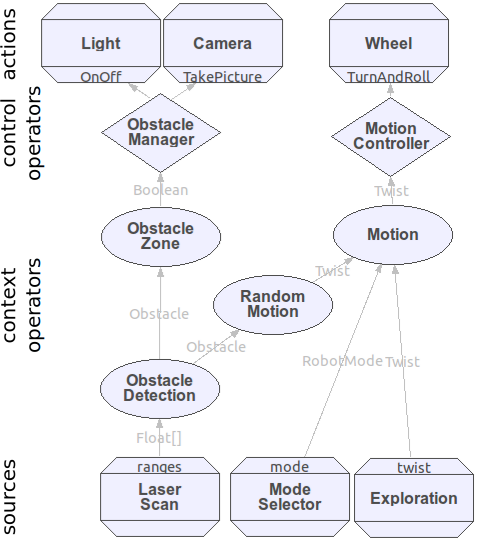
\includegraphics[width=.7\linewidth]{diaspec-graph}
  \caption{The case study decomposed into the different type of
    components of \diaspec{}}
\label{fig:diaspec-graph}
\end{figure}

\paragraph*{Reusing existing components}
We assume no previous \diaspec{} application and thus no \diaspec{}
component to reuse.

\paragraph*{Listing capabilities}
Our robot comes with a range-finder type laser scanner, a light
projector, a camera, and a set of wheels. We are reusing the
\emph{exploration} capability developed by the Bosch robotics research
group.\footnote{\url{http://www.ros.org/wiki/explore}} This capability
is based on a well-known frontier-based exploration
algorithm~\cite{Yamau98a}. In this algorithm the exploration is
composed of two steps: a motion toward a location and a new
observation of the environment at this location. The location is
chosen among a set of candidate locations on the frontier between
explored and unexplored space. This capability is exactly what we need
for the robot's exploration mode. From all these capabilities, we
identify:
\begin{itemize}
\item a \ct{LaserScan} entity class with a \ct{ranges} source
  providing laser ranges from the sensor which can be deactivated when
  the robot is in exploration mode;\footnote{it is important to note
    that the application is not going to deactivate the hardware-level
    sensor (which is used in the two modes) but only the
    application-level source (which is only used in the random mode).}
\item A \ct{ModeSelector} entity that provides a graphical interface
  for the operator to choose the robot's current mode.
\item an \ct{Exploration} entity that provides a source of twists for
  the robot;
\item a \ct{Light} and \ct{Camera} entities that respectively take
  pictures and enlighten the neighborhood on request;
\item a \ct{Wheel} entity that can turn or roll on request;
\end{itemize}

\paragraph*{Identifying main context operators}
The most important activity of our robot is to move. Therefore we
introduce a \ct{Motion} context operator that produces a twist,
representing the robot's motion. Because our robot takes pictures and
turns on its projector when it is in a zone with obstacles, we
introduce an \ct{ObstacleZone} context operator that indicates whether
or not some obstacles are in the neighborhood.

\paragraph*{Decomposing into lower-level pieces}
The \ct{Motion} context operator produces a twist based on which mode
is currently selected and on the twist values coming from both modes.
The currently selected mode is directly provided by the
\ct{ModeSelector} entity. We introduce a \ct{RandomMotion} context
operator that produces random twists. The twist for the exploration
mode is directly provided by the \ct{Exploration} entity. Both the
\ct{ObstacleZone} and \ct{RandomMotion} context operators need the
information about nearby obstacles. We thus introduce the
\ct{ObstacleDetection} context operator to indicate the proximity of
an obstacle.

\paragraph*{Identifying control operators}
The \ct{MotionController} control operator takes information from the
\ct{Motion} context operator and transmit this information to the
\ct{Wheel} entity. The \ct{ObstacleManager} control operator takes
information from the \ct{ObstacleZone} context operator and triggers the
light and takes a picture with the camera.

\paragraph*{Identifying data types}
We have already seen that our application uses the notion of twist to
indicate motion. A twist can be defined as a pair of vector which
represent the linear and angular velocity. The robot current mode is
represented as an enumeration of the \ct{RANDOM} and \ct{EXPLORATION}
names. The \ct{ObstacleDetection} context operator provides an
\ct{Obstacle} data type containing both a boolean to indicate if an
obstacle is in front of the robot and a set of float numbers (the
ranges) as provided by the laser scan giving details about the
neighborhood.

\subsection{Describing with \diaspec{}}

Once the application is decomposed using the different component
types, the transcription to the \diaspec{} design language is
straightforward. Listing~\ref{listing:design} gives an extract of the
case study transcription.

\lstinputlisting[float,language=diaspec, numbers=left,
breakatwhitespace=true,%
caption={An extract of the description of the robotics application
  with the \diaspec{} design language}%
,label={listing:design}]%
{code/design.diaspec}

In this listing, the \ct{entity}, \ct{context}, and \ct{controller}
keywords are respectively used to introduce a new entity class, a new
context operator, and a new control operator. For this application, we
decide to reuse the \ct{Twist} data type of the ROS middleware which
is illustrated in line~\ref{design:import}.

Additionally to the description of an operator's input sources, the
\diaspec{} language allows each operator to describe a set of
\emph{interaction contracts} that coordinate these input sources. An
interaction contract is a tuple that describes an \emph{activation
  condition} indicating which input sources can activate the operator
and a \emph{reaction} indicating what to do as a result of the
activation condition.\footnote{Previous work~\cite{Cass11a} also
  includes in the tuple a set of \emph{data requirements} indicating
  the additional input sources that can be used for a particular
  activation condition. This is not used in this case study.} The
\ct{interaction} keyword is used to introduce an interaction contract.
For example, the \ct{ObstacleDetection}'s interaction contract
(Listing~\ref{listing:design}, line~\ref{design:interaction})
indicates that this context operator always publishes a data when it
receives information from the laser scan.

In this section we saw how to design a robotics application using
the SCC architectural pattern and the \diaspec{} design language. Both
the pattern and the language help decomposing an application in well
defined components. Both make it easy to reuse as much as possible
from the underlying middleware and existing applications. In the next
section we discuss how to implement a robotics application with our
approach.

%%% Local Variables:
%%% mode: latex
%%% coding: utf-8
%%% TeX-master: "dslrob"
%%% TeX-PDF-mode: t
%%% ispell-local-dictionary: "english"
%%% End:

% LocalWords:  boolean
